\documentclass[10pt]{beamer}
%\documentclass[10pt, handout]{beamer}
%\setbeameroption{show notes}

%\documentclass[10pt, a4paper]{article}
%\usepackage{beamerarticle}




\mode<article>{
	
	\usepackage{hyperref}
	
}
\mode<presentation>{
	
	\usetheme{Antibes}
	\usefonttheme{professionalfonts} 
	\usefonttheme{serif} % default family is serif
	
	%\usecolortheme{spruce} %зеленая, плохой цвет в заголовках 
	%\usecolortheme{albatross} %синяя, пхоло виден черный цвет
	
}

\newcommand{\MP}[1]{\mode<presentation>{#1} }
\newcommand{\MA}[1]{\mode<article>{#1} }

\newcommand{\ABS}[1]{\left| #1 \right|}
%\newcommand{\ABS}[1]{\mid #1 \mid}

\newcommand{\HREF}[2]{{\color{blue}\underline{\href{#1}{#2}}}}

\setbeamertemplate{caption}[numbered]


%\usepackage[T2A]{fontenc}
%\usepackage[utf8]{inputenc}
%\usepackage[russian]{babel}
%\usepackage{amsmath} %математические формулы



\usepackage{ifthen}

\usepackage{tikz}
\usetikzlibrary{arrows.meta}

\usepackage{fp}
\usepackage{tikz-3dplot}
\usepackage{environ}
\usepackage{animate}




\usepackage{xcolor}
%\usepackage[left=20mm,right=20mm,top=20mm,bottom=20mm,a4paper]{geometry} %поля

\usepackage{amsmath} %математические формулы


\usepackage[e]{esvect}  %Красивая стрелочка вектора
%\let\oldvv\vv
\newcommand{\VV}[1]{\vv{#1\mathstrut}}



\usepackage{graphicx} %работа с каритнками


\usepackage{multimedia}

%Для XeLatex/+
\usepackage{polyglossia}
\setdefaultlanguage{russian}
\setotherlanguage{english}
\setkeys{russian}{babelshorthands=true}


\usepackage{fontspec}

\setmainfont{Times New Roman} [Script=Cyrillic, Mapping=tex-text,]
\setsansfont{Arial} [Script=Cyrillic, Mapping=tex-text,]
\setmonofont{Courier New} [Script=Cyrillic, Mapping=tex-text,]



\usepackage{unicode-math}
%\setmathfont{TeX Gyre Termes Math}

%\setmainfont{CMU Serif}[Script=Cyrillic, Mapping=tex-text,]
%\setsansfont{CMU Sans Serif}[Script=Cyrillic, Mapping=tex-text,]
%\setmonofont{CMU Typewriter Text}[Script=Cyrillic, Mapping=tex-text,]


%-----------------


%\usepackage{caption}
%\DeclareCaptionLabelSeparator{dot}{~---~}            %Разделитель номер рисунка
%\captionsetup[figure]{justification=centering,labelsep=dot, format=plain}                        %Подпись рис. центр
%\captionsetup[table]{justification=raggedleft,labelsep=dot, format=plain, singlelinecheck=false} %Подпись табл. слева
%\captionsetup[lstlisting]{justification=raggedleft,labelsep=dot, format=plain, singlelinecheck=false}                     %Подпись рис. центр

\usepackage{indentfirst} %отступ первой строки


\usepackage[svgnames]{xcolor}


%\usepackage{showframe}


%\usepackage{tikz}

%\usepackage[hidelinks]{hyperref}%ссылки внутри документа \ref


\setlength\abovecaptionskip{-2pt}
%\setlength\belowcaptionskip{-14pt}

\setbeamerfont{caption}{size=\scriptsize}


\def\sectionname{Раздел}
\def\subsectionname{Подраздел}


\newcommand{\TC}[3]
{
	
	
	\begin{columns}
		\begin{column}{#1\textwidth}
			#2
		\end{column}
		\begin{column}{\fpeval{1-#1}\textwidth}
			#3
		\end{column}
	\end{columns}
}

\newcommand{\TCT}[3]
{
	
	\begin{columns}[T]
		\begin{column}{#1\textwidth}
			#2
		\end{column}
		\begin{column}{\fpeval{1-#1}\textwidth}
			#3
		\end{column}
	\end{columns}
}


\newcommand{\FRAME}[2]{
	\begin{frame}
		\frametitle{#1}
		#2
	\end{frame}
}

\newcommand{\FIG}[3]
{
	\begin{figure}
		\centering
		\includegraphics[width=#3]{#1}
		\caption{#2}
	\end{figure}
}

\newcommand{\vect}[1]{\overrightarrow{#1}}


\usepackage{newfile}

\edef\LectionNumber{0}

\let\oldsection\section
\let\oldsubsection\subsection


\AtBeginDocument
{
	\newoutputstream{CONTENT}
	\openoutputfile{\LectionNumber .gvr}{CONTENT}
	
	\expandafter\addtostream{CONTENT}{\noindent\textbf{\Large\inserttitle}\unexpanded{\setcounter{SEC}{0}}\par}
}

\renewcommand{\section}[1]{
	\oldsection{#1}
	\expandafter\addtostream{CONTENT}{\noindent\hspace{2ex}\unexpanded{\hbox{\large\stepcounter{SEC}\theSEC ~ #1}}\par}
}

\renewcommand{\subsection}[1]{
	\oldsubsection{#1}
	\expandafter\addtostream{CONTENT}{\noindent\hspace{6ex}\unexpanded{\stepcounter{SUB}\theSUB ~ #1}\par}
}

%\renewcommand{\section}[1]{\MMM{#1}}

%\edef\subsection#1
{
	%\noexpand\subsection{#1}
	%
}


\author{Гаврилов Андрей Геннадьевич}
\institute{Кафедра Информационных технологий и вычислительных систем \\МГТУ~<<СТАНКИН>>}
\lecture{История компьютерной графики}{kghistory}\subtitle{Компьютерная графика}



\graphicspath{{Images/}{Images/L3}}

\date{\today}

\renewcommand{\LectionNumber}{3}
\title{Лекция 3 \\Преобразования точек на плоскости}


\usepackage{standalone}

\setbeamersize
{
	text margin left=0.5cm,
	text margin right=0.5cm
}

\usepackage{comment}


%	\transduration{2}
%   \transfade

 \begin{document}
 		 
	\makeatletter
\defbeamertemplate*{title page}{my theme}
{
	
	\hfill
	
	\begin{beamercolorbox}[wd=.9\paperwidth,center,]{title}%
		
	\end{beamercolorbox}%	
	
	\vbox to 1em {}
	
	\begin{beamercolorbox}[wd=.9\paperwidth,center,]{title}%
		\usebeamerfont{subtitle}%
		\hfill
		
		\insertsubtitle
		
		\usebeamerfont{title}%
		\inserttitle{} \\[0.5em]
		
		
		
	\end{beamercolorbox}%	
	\hfill\hfill
	
	\begin{beamercolorbox}[wd=.9\paperwidth,center,]{}%
		\usebeamerfont{author}%
		\hfill \\[0.5em]
		\insertauthor{}
		
		\vbox to 1em{}
		\usebeamerfont{institute}%
		\insertinstitute {}
		
		\vbox to 1em{}			
		{\; }\insertshortdate{}
		
	\end{beamercolorbox}%	
	\hfill\hfill
	
	\vbox to 5em{}
	
	
}
\defbeamertemplate*{footline}{my theme}{
	\leavevmode%
	\hbox{%
		\begin{beamercolorbox}[wd=.25\paperwidth,ht=2.25ex,dp=1ex,center]{author in head/foot}%
			\usebeamerfont{author in head/foot}%
			\insertauthor~~\beamer@ifempty{\insertshortinstitute}{}
		\end{beamercolorbox}%
		\begin{beamercolorbox}[wd=.65\paperwidth,ht=2.25ex,dp=1ex,center]{title in head/foot}%
			\usebeamerfont{title in head/foot}\insertshortinstitute
		\end{beamercolorbox}%
		\begin{beamercolorbox}[wd=.1\paperwidth,ht=2.25ex,dp=1ex,right]{date in head/foot}%
			\usebeamerfont{date in head/foot}\hspace*{2em}
			\insertframenumber{} / \inserttotalframenumber\hspace*{2ex}
	\end{beamercolorbox}}%
}



\makeatother






%float page top aligment
\makeatletter
\setlength{\@fptop}{0pt}
\setlength{\@fpbot}{0pt plus 1fil}
\makeatother

\begin{comment}
\end{comment}



    
    \begin{frame}[plain]
    	
    	
    	\centering
    	Трансляция презентации (во время очных лекций).     
    		
    	
\includegraphics[width=0.5\textwidth]{qr.png} \\ ~ \\
    	
    	
    	При просмотре презентации в PDF для отображения анимаций на слайдах необходимо использовать Acrobat Reader, KDE Okular, PDF-XChange или Foxit Reader.

    \end{frame}
	
	
	\frame{\maketitle}
	
	
	
	\begin{frame}{План лекции}
		\tableofcontents
	\end{frame}
	
	\section{Матрицы}
	\frame{\sectionpage}
	
	\begin{frame}{Матрицы и операции над ними}
		$\mathbf M =
		\begin{pmatrix} a_{11} & a_{12} & \cdots & a_{1n}
			\\a_{21} & a_{22} & \cdots & a_{2n}
			\\ \vdots & \vdots & \ddots & \vdots
			\\ a_{m1} & a_{m2} & \cdots & a_{mn}
		\end{pmatrix} 
		$ --- матрица размером $m \times n$ \\
		$\mathbf E = \begin{pmatrix} 1 & 0 & \cdots & 0 \\ 0 & 1 & \cdots & 0 \\ \vdots & \vdots & \ddots & \vdots \\ 0 & 0 & \cdots & 1 \end{pmatrix}$ --- единичная матрица
		
		$\mathbf A = \begin{pmatrix}
			a_1 & a_2 & \ldots & a_n
		\end{pmatrix}$ --- матрица-строка
		
		$\mathbf B = \begin{pmatrix}
			b_1 \\ b_2 \\ \vdots \\ b_n
		\end{pmatrix}$ --- матрица-столбец	
		
	\end{frame}
	
	\begin{frame}{Транспонирование матрицы}
		
		Если $\mathbf B=\mathbf A^T$, то $a_{ij}=b_{ji}$ \\ ~ \\
		
		$\mathbf M ^ {TT} = \mathbf M$ \\ ~ \\
		
		\TC{0.5}
		{
			$\mathbf M =
			\begin{pmatrix} a_{11} & a_{12} & \cdots & a_{1n}
				\\a_{21} & a_{22} & \cdots & a_{2n}
				\\ \vdots & \vdots & \ddots & \vdots
				\\ a_{m1} & a_{m2} & \cdots & a_{mn}
			\end{pmatrix} 
			$
			
			$\mathbf M^T =
			\begin{pmatrix} a_{11} & a_{21} & \cdots & a_{m1}
				\\a_{12} & a_{22} & \cdots & a_{m2}
				\\ \vdots & \vdots & \ddots & \vdots
				\\ a_{1n} & a_{2n} & \cdots & a_{mn}
			\end{pmatrix} 
			$ 
		}
		{
			$\mathbf A = \begin{pmatrix}
				a_1 & a_2 & \ldots & a_n
			\end{pmatrix}$ \\
			$\mathbf A^T = \begin{pmatrix}
				a_1 \\ a_2 \\ \vdots \\ a_n
			\end{pmatrix}$
		}
		
		
		
		
		
	\end{frame}
	
	\begin{frame}{Сложение матриц}
		
		$
		\begin{pmatrix} a_{11} & a_{12} & \cdots & a_{1n}
			\\a_{21} & a_{22} & \cdots & a_{2n}
			\\ \vdots & \vdots & \ddots & \vdots
			\\ a_{m1} & a_{m2} & \cdots & a_{mn}
		\end{pmatrix} 
		+
		\begin{pmatrix} b_{11} & b_{12} & \cdots & b_{1n}
			\\b_{21} & b_{22} & \cdots & b_{2n}
			\\ \vdots & \vdots & \ddots & \vdots
			\\ b_{m1} & b_{m2} & \cdots & b_{mn}
		\end{pmatrix} 
		=$
		$
		=
		\begin{pmatrix} a_{11}+b_{11} & a_{12}+b_{12} & \cdots & a_{1n}+b_{1n}
			\\a_{21}+b_{21} & a_{22}+b_{22} & \cdots & a_{2n}+b_{2n}
			\\ \vdots & \vdots & \ddots & \vdots
			\\ a_{m1}+b_{m1} & a_{m2}+b{m2} & \cdots & a_{mn}+b{mn}
		\end{pmatrix} 
		$
		
	\end{frame}
	
	\begin{frame}{Умножение матриц}
		\TC{0.55}
		{
			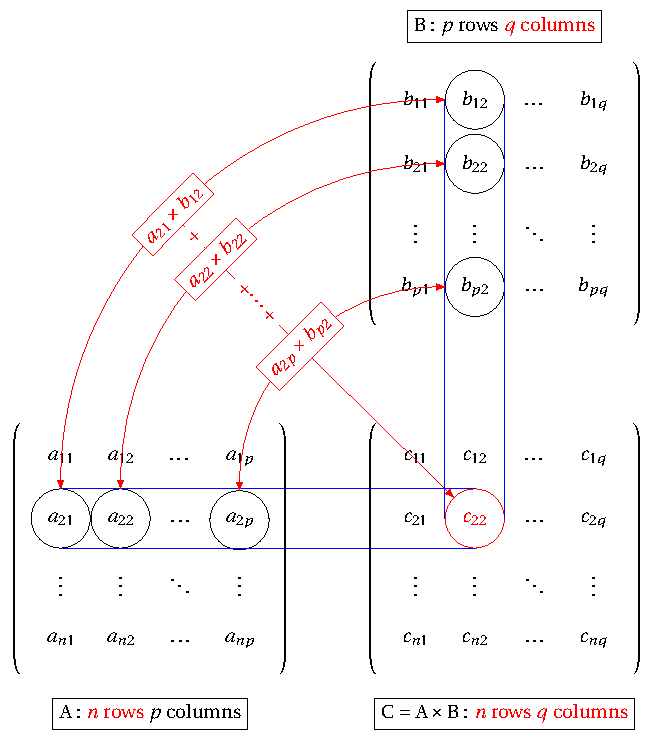
\includegraphics[width=\textwidth]{../L3/matrix-multiplication.pdf}
		}
		{
			$\mathbf C = \mathbf A \mathbf B$\\
			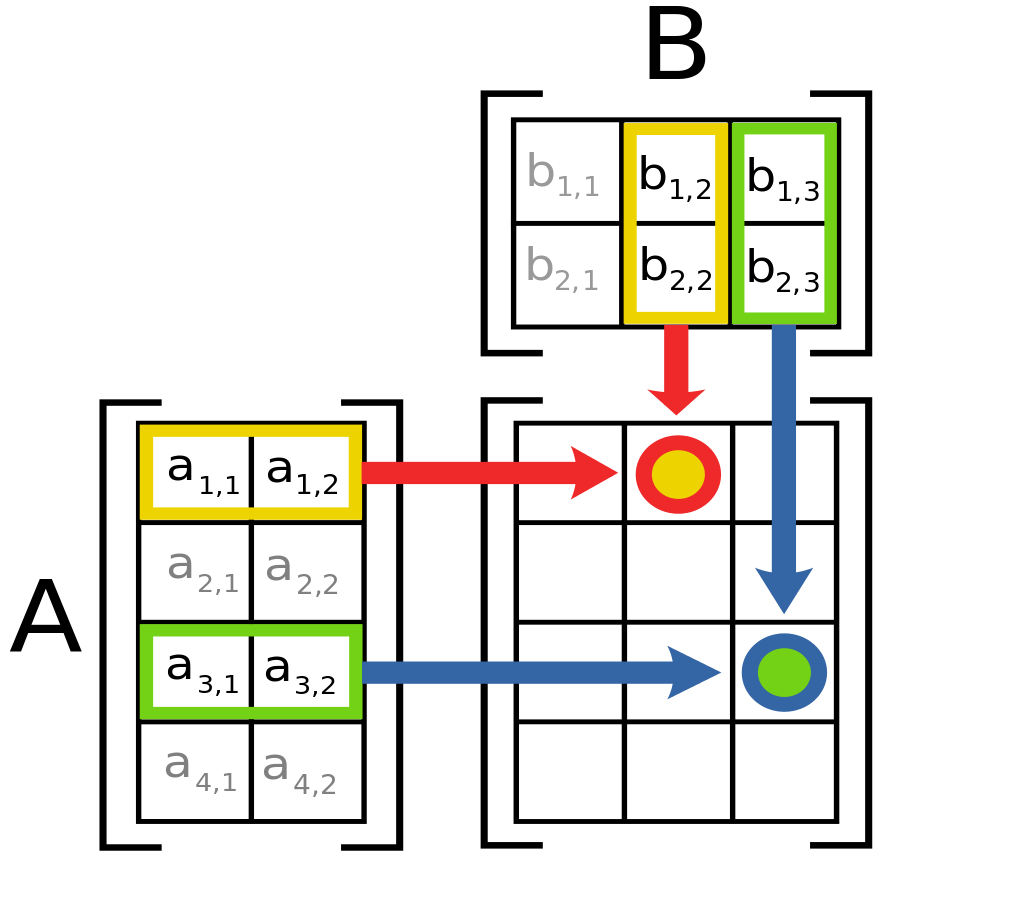
\includegraphics[width=\textwidth]{../L3/Matrix_multiplication_diagram_2.svg.png}
		}
		
	\end{frame}
	
	\begin{frame}{Обратная матрица}
		
		\begin{center}
			
			$k\cdot\displaystyle\frac{1}{k}=1$ \ \ \ \ \   $\mathbf M\cdot \mathbf M^{-1}=\mathbf E$
			
		\end{center}
		
		\TCT{0.5}
		{
			$\mathbf M^{-1}$ --- обратная матрица \\ ~ \\
			
			$\left[ \mathbf A^{-1}\right]^{-1} = \mathbf A$ \\ ~ \\
			
			$ \left( \mathbf{AB} \right) ^{-1}=\mathbf A^{-1}\mathbf B^{-1}$ \\~\\
			
			$ \left[\mathbf A^T\right]^{-1}  = \left[\mathbf A^{-1}\right]^{T} $
			
			
			
		}
		{
			$\mathbf E = \begin{pmatrix} 1 & 0 & \cdots & 0 \\ 0 & 1 & \cdots & 0 \\ \vdots & \vdots & \ddots & \vdots \\ 0 & 0 & \cdots & 1 \end{pmatrix}$
			
			
		}	
		
		
	\end{frame}
	
	\begin{frame} {Определитель матрицы}
		$\det(\mathbf A), \quad |\mathbf A|, \quad \Delta(\mathbf A) $ \\ ~ \\
		
		Для матрицы 2х2: \\
		$\begin{vmatrix} a & c \\ b & d \end{vmatrix}=ad-bc$ \\ ~ \\
		Для матрицы 3x3: \\
		$\begin{vmatrix} a_{11} & a_{12} & a_{13} \\ a_{21} & a_{22} & a_{23} \\ a_{31} & a_{32} & a_{33} \end{vmatrix} =
		a_{11}\begin{vmatrix}    a_{22} & a_{23} \\  a_{32} & a_{33} \end{vmatrix}-a_{12}\begin{vmatrix}    a_{21} & a_{23} \\  a_{31} & a_{33} \end{vmatrix}+a_{13}\begin{vmatrix}    a_{21} & a_{22} \\  a_{31} & a_{32} \end{vmatrix} = $\\ 
		$
		= a_{11}a_{22}a_{33} - a_{11}a_{23}a_{32}  - a_{12}a_{21}a_{33}+ a_{12}a_{23}a_{31} + a_{13}a_{21}a_{32} - a_{13}a_{22}a_{31} $
		
		
	\end{frame}
	
	\section{Проекции и их виды}
	
	\frame{\sectionpage}
	\subsection{Виды проекций}
	

	
  %https://www.youtube.com/watch?v=E4UHbRW1bFM
  %https://www.youtube.com/watch?v=d4kt2qFl0ac
	
	\begin{frame}
		\frametitle{Виды проекций}
		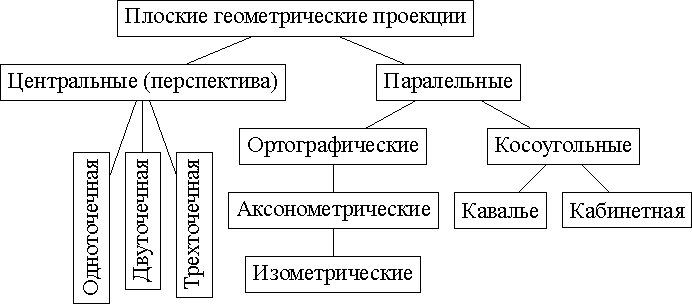
\includegraphics[width=\textwidth, page=1]{Images/L3/projections.pdf}
	\end{frame}
	
	\FRAME{Виды проекций}
	{
		\centering
		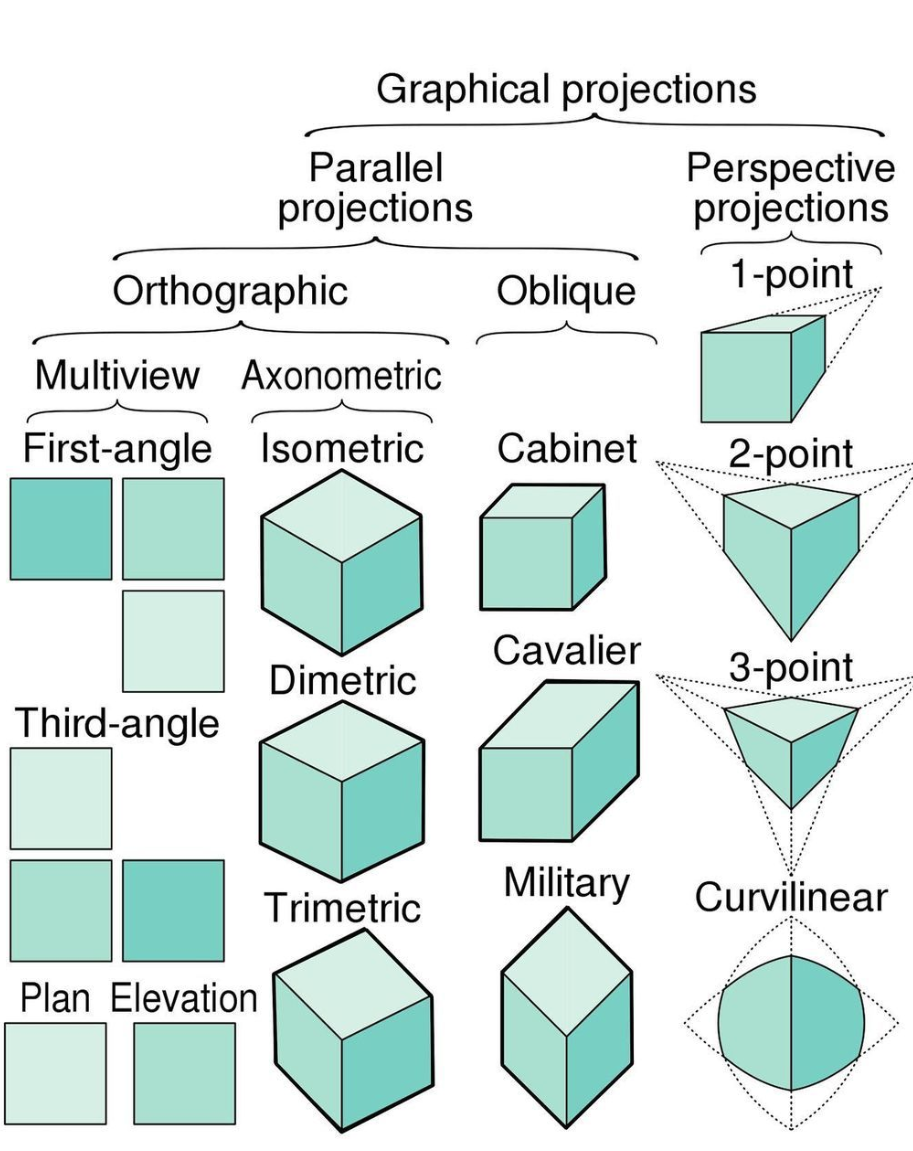
\includegraphics[height=200pt]{Screenshot 2024-02-29 232325.png}
	}
	

    \begin{frame}
    	\frametitle{Два основных вида проекций}
    	
    	\TCT{0.5}
    	{
    		\centering
    		
    		\textbf{Центральная проекция} \\ ~ \\
    		
    		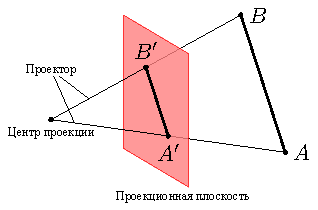
\includegraphics[width=\textwidth]{Images/L3/centralproj.pdf}
    	}
    	{
    		\centering
    		
    		\textbf{Паралельная проекция}  \\ ~ \\
    		
    		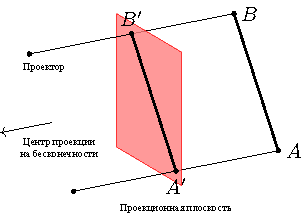
\includegraphics[width=\textwidth]{Images/L3/parproj.pdf}
    	}
    	
    	
    \end{frame}
    
    \subsection{Перспективные проекции}
    
    \FRAME{Перспектива}
    {
    	\centering
    	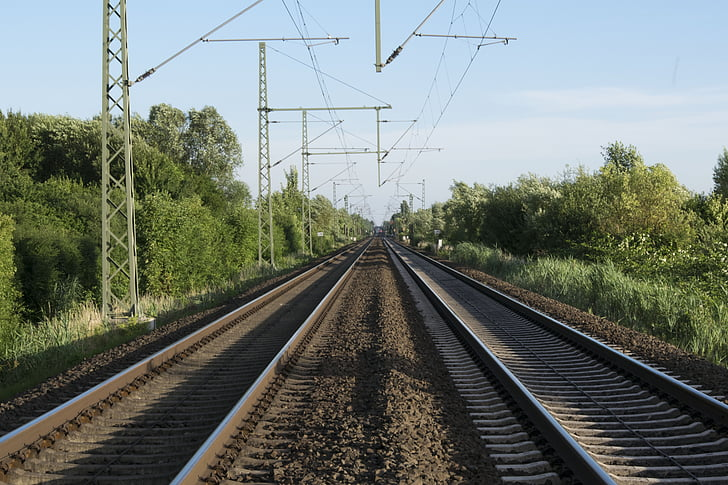
\includegraphics[width=0.85\textwidth]{train-tracks-railroad-transportation-preview.jpg}
    }
    
    \FRAME{Двухточечная перспектива}
    {
    	\centering
    	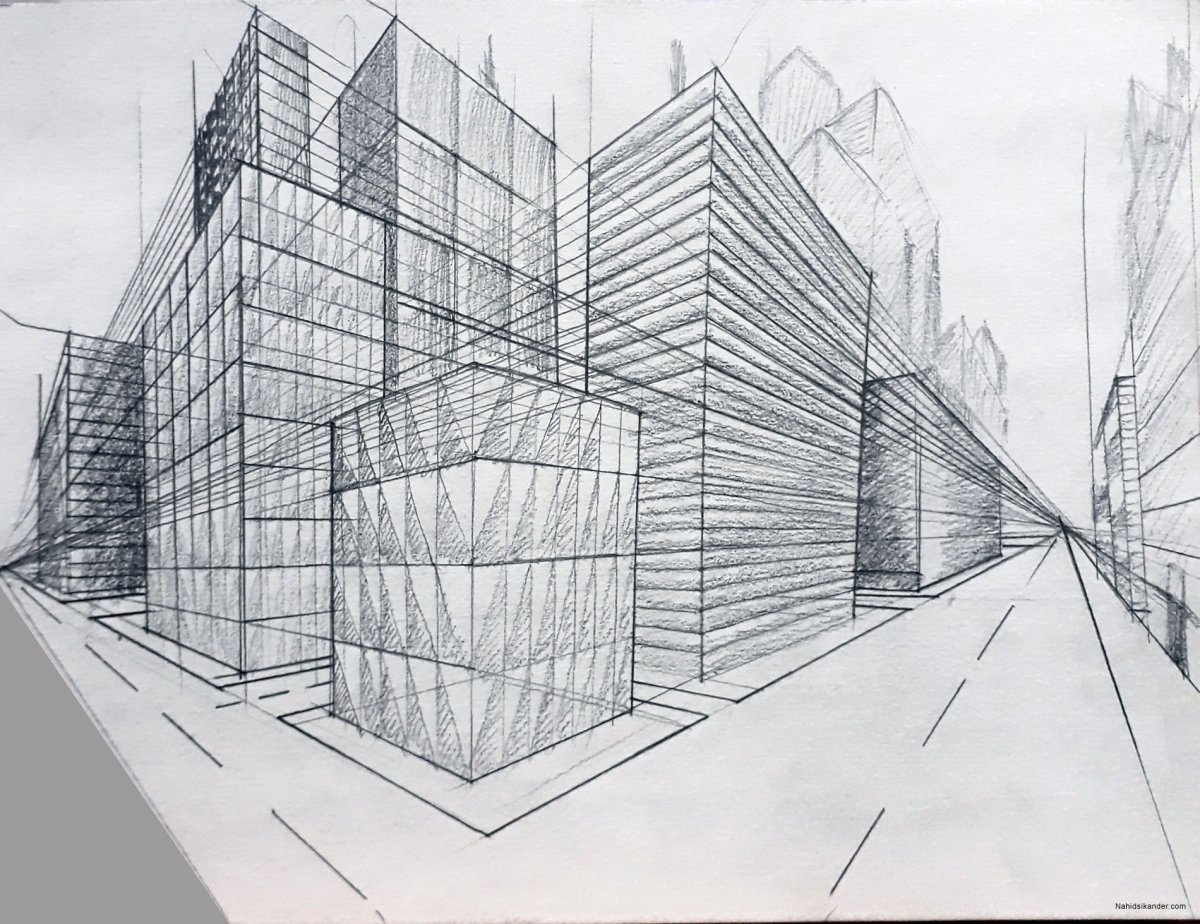
\includegraphics[width=0.7\textwidth]{1670050141_8-indasil-club-p-risunok-perspektiva-dlya-nachinayushchikh-9.jpg}
    }
    
   
    
    \FRAME{Трёхточечная перспектива}
    {
    	\centering
    	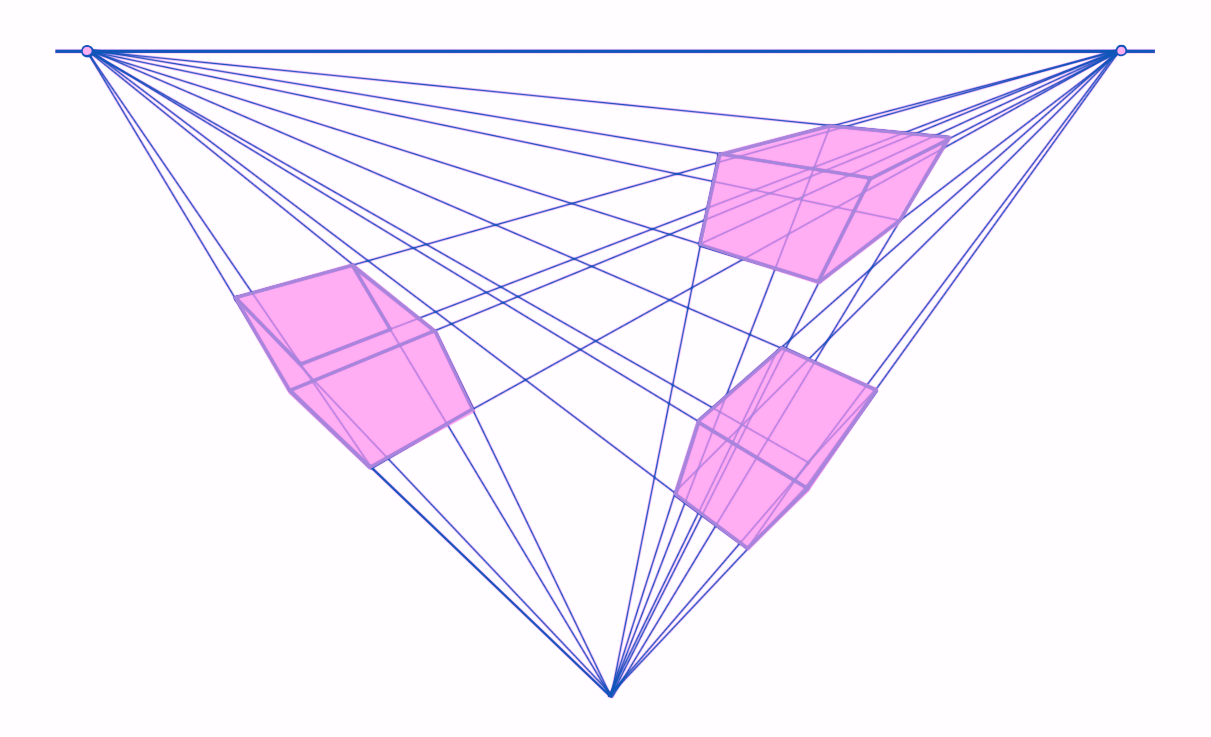
\includegraphics[width=0.9\textwidth]{8a8420d9-84c8-5ef2-a90d-76981bc7f72d.png}
    }
    
    \FRAME{Обратная перспектива}
    {
    	
    	\centering
    	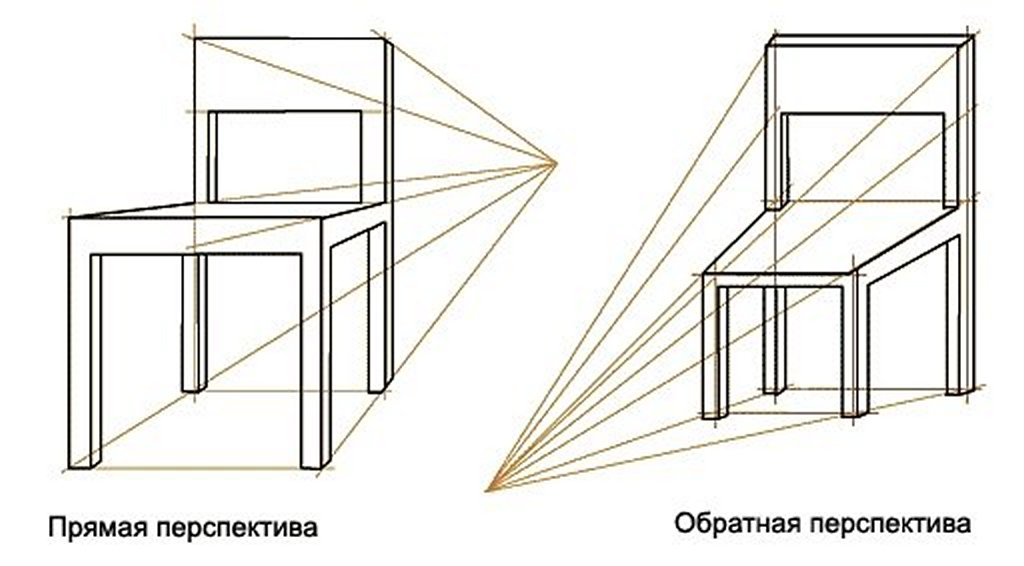
\includegraphics[width=\textwidth]{5.jpg}
    }
    
    \FRAME{Обратная перспектива}
    {
    	\TC{0.5}
    	{
    		\centering
    		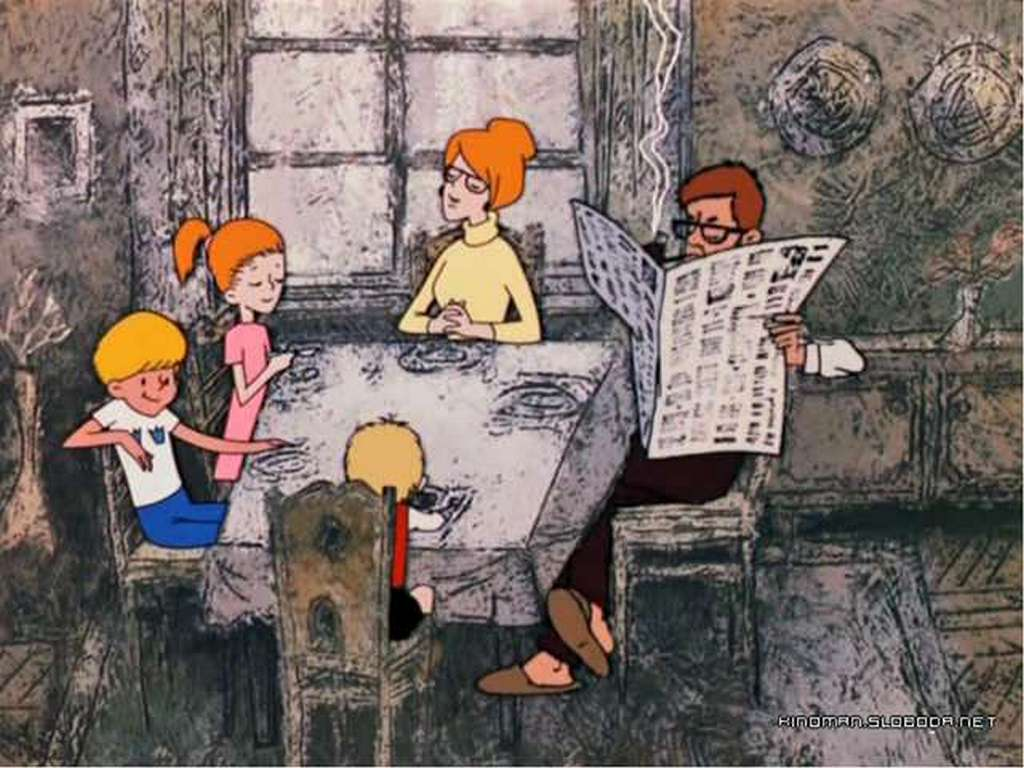
\includegraphics[width=\textwidth]{3.jpg}
    	}
    	{
    		\centering
    		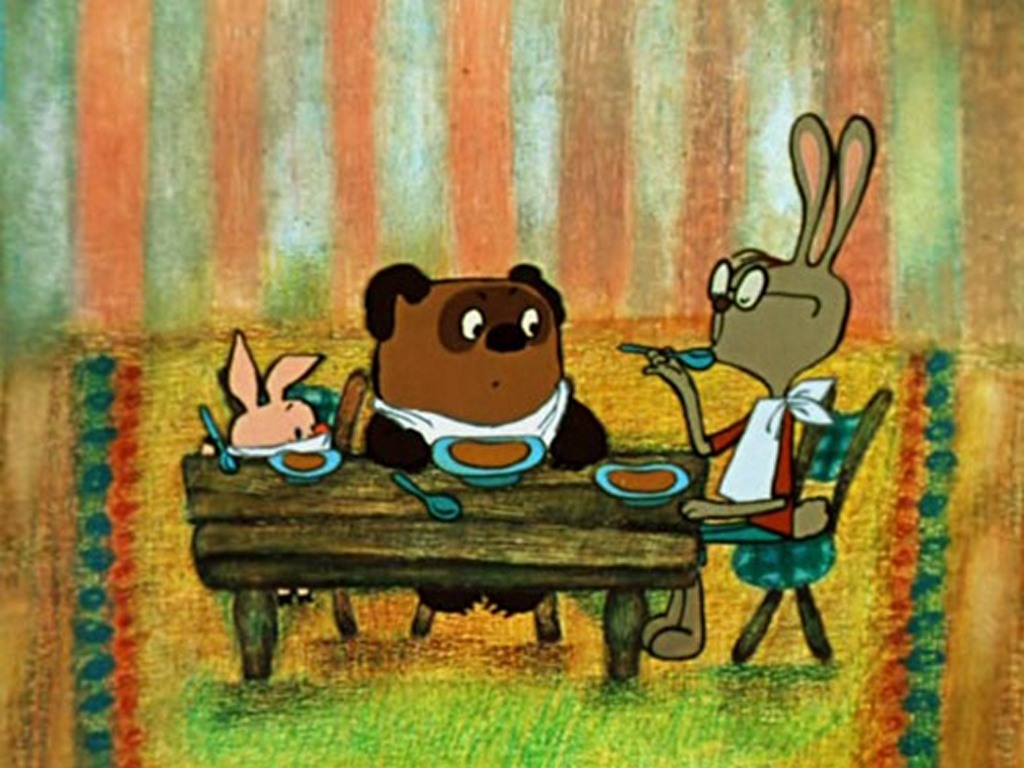
\includegraphics[width=\textwidth]{1.jpg}
    	} 	
    	
    	\centering 
    	
    	В советской мультипликации
    }
    
    \FRAME{Обратная перспектива}
    {
    	\TCT{0.5}
    	{
    		\centering
    		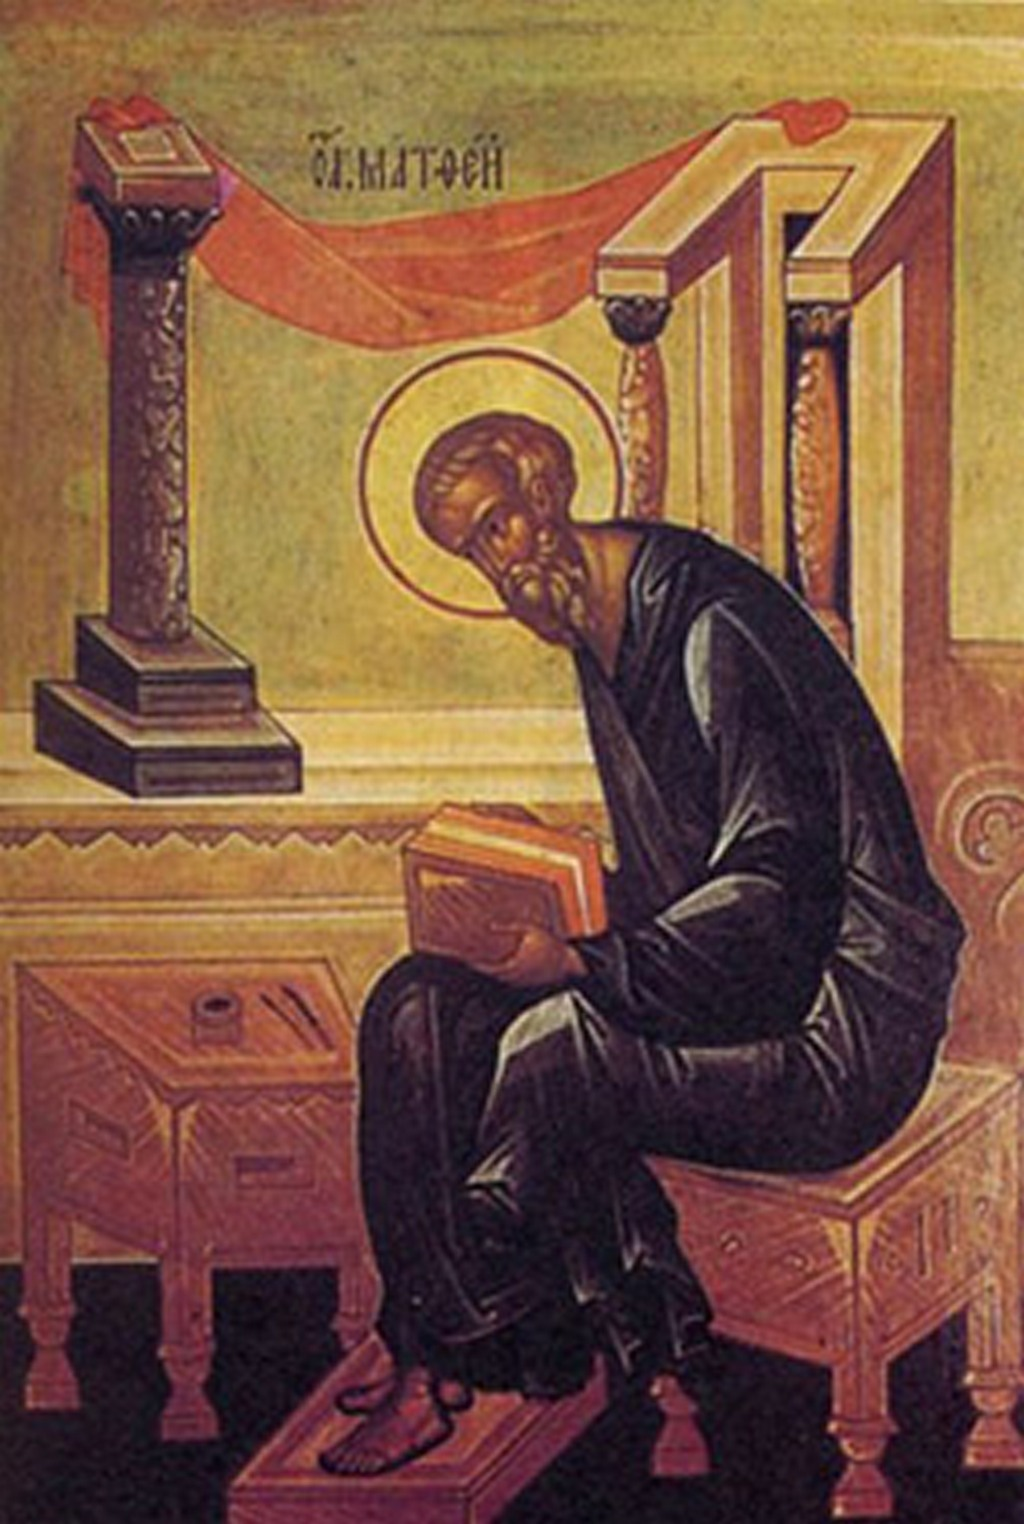
\includegraphics[height=160pt]{4.jpg}
    		
    		Апостол и евангелист Матфей
    	}
    	{
    		\centering
    		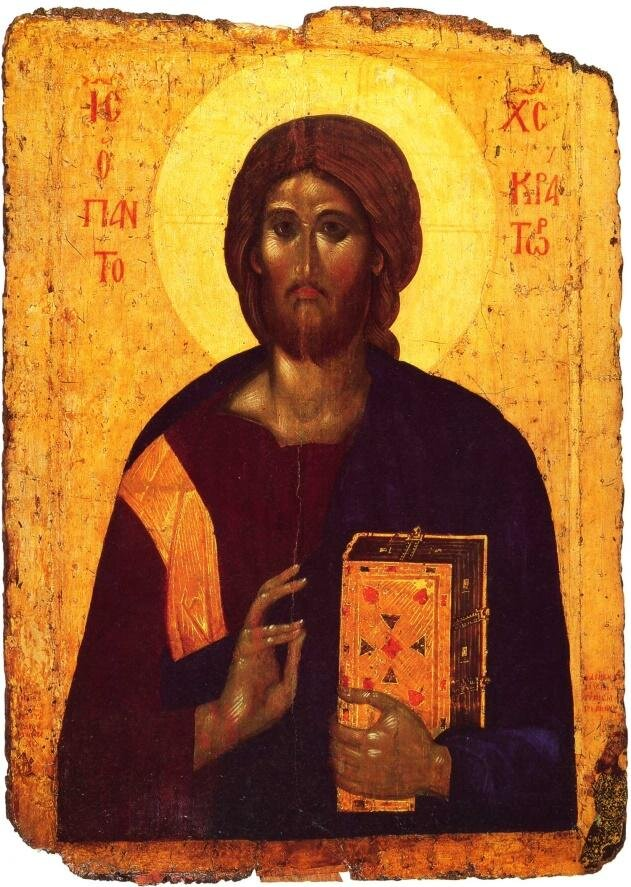
\includegraphics[height=160pt]{scale_1200.jpg}
    		
    		Спас Вседержитель (1363 г.)
    	} 	
    }
    
    \subsection{Вычисление центральной проекции}
    
    \FRAME{Координатная система экрана}
    {
    	\centering
    	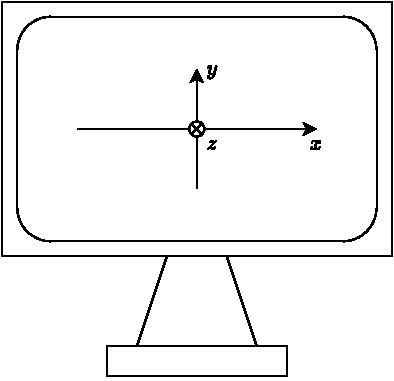
\includegraphics[width=0.5\textwidth]{screen.pdf}
    }
    

   \begin{frame}{Проекция точки на экран (1)}\label{slide:projection}
	
		\TC{0.5}
		{
			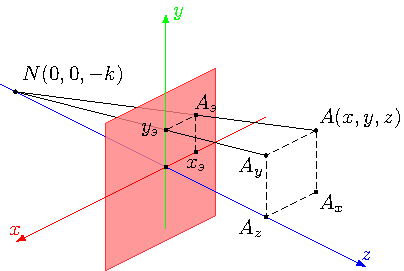
\includegraphics[width=\textwidth]{centralproj1.pdf}
		}
		{
			\def\ekr{\text{\textit{э}}}
			$A(x,y,z) \rightarrow A_\ekr (x_\ekr, y_\ekr) $ \\ ~ \\
			
			1. $\triangle A_yA_zN \sim \triangle A_{\ekr y}ON$   \\ ~ \\
			
			\pause
			
			2. $\displaystyle \frac{y}{z+k} = \frac {y_\ekr}{k}, \ \frac{x}{z+k} = \frac {x_\ekr}{k}$ \\ ~ \\
			
			
			\pause
			
			3. \fbox{$\displaystyle y_\ekr=\frac{ky}{z+k}, \ x_\ekr=\frac{kx}{z+k}$}	
			
		}
		
	\end{frame}
    
    
    \begin{frame}{Проекция точки на экран (2)}
    	\TC{0.5}
    	{
    		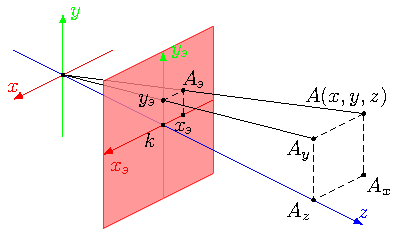
\includegraphics[width=\textwidth]{centralproj2.pdf}
    	}
    	{
    		\def\ekr{\text{\textit{э}}}
    		
    		$A(x,y,z) \rightarrow A_\ekr (x_\ekr, y_\ekr) $ \\ ~ \\
    		
    		
    		\fbox{$\displaystyle y_\ekr=\frac{ky}{z}, \ x_\ekr=\frac{kx}{z}$}	
    		
    	}
    \end{frame}
    
    \section{Двумерные преобразования}
    
    \frame{\sectionpage}
    
    \subsection{Перенос}
    
    \FRAME{Перенос точки}
    {
    	\TC{0.5}
    	{
    		\centering
    		\only<1>{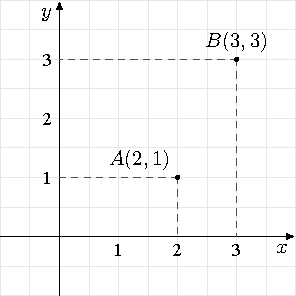
\includegraphics[page=1]{translate.pdf}
    		}\only<2->{\includegraphics[page=2]{translate.pdf}}
    		
    	}
    	{
    		$A \rightarrow B $ \\~\\
    		
    		\pause
    		
    		$\vv{B} = \vv{A} + \vv{AB}$  \\~\\    	
    		
    		\pause
    		
    		$\vv{AB} \equiv \vv{R} $ --- вектор переноса
    		
    		\begin{block}{Перенос точки $A$ на вектор $\vv{R} $ }
    			$\vv{B} = \vv{A} + \vv{R} = $ \\ $\quad \quad =(A_x+R_x, \ A_y+R_y, \ A_z+R_z) $
    		\end{block}
    		
    	}
    	
    }
    
    \subsection{Масштабирование}
    
    \FRAME{Равномерное масштабирование}
    {
    	\TC{0.5}
    	{
    		\centering
    		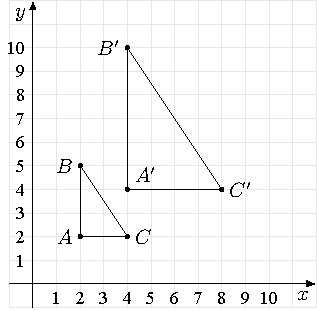
\includegraphics[]{scale.pdf}
    		
    		
    	}
    	{
    		$\triangle ABC \rightarrow \triangle A'B'C' $ \\~\\
    		
   		   		
    		\pause
    		
    		$$\vv{A'}=k\cdot\vv{A}, \ \vv{B'}=k\cdot\vv{B}, \ \vv{C'}=k\cdot\vv{C}.$$
    		
    		
    		
    	}
    	
    }
    
    \FRAME{Неравномерное масштабирование}
    {
    	\TC{0.5}
    	{
    		\centering
    		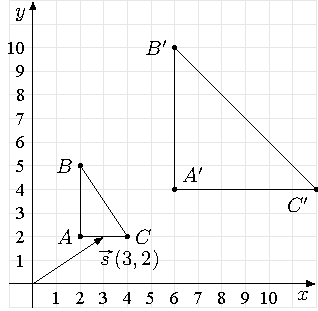
\includegraphics[]{scale2.pdf}
    		
    		
    	}
    	{
    		$\triangle ABC \rightarrow \triangle A'B'C' $ 
    		$\triangle ABC \nsim \triangle A'B'C' $ \\ ~ \\
    		
    		\pause
    		
    		$A \rightarrow A' : A'=(A_xs_x, A_ys_y) $ \\ ~ \\
    		
    		\pause
    		
    		\begin{block}{Масштабирование точки $(x,y)$ по вектору $\vv{s}$ }
    			 $$  
    			\begin{pmatrix}
    				x' \\ y'
    			\end{pmatrix}   
    			=    		
    			\begin{pmatrix}
    				s_x & 0 \\
    				0   & s_y  
    			\end{pmatrix} 
    			\cdot     
    			\begin{pmatrix}
    				x \\ y
    			\end{pmatrix} 		   
    			$$
    		\end{block}    		
    		
    		
    	}
    	
    }
    
    
    \subsection{Поворот}
    
    \begin{frame}{Поворот точки}
    	
    	\TC{0.4}
    	{
    		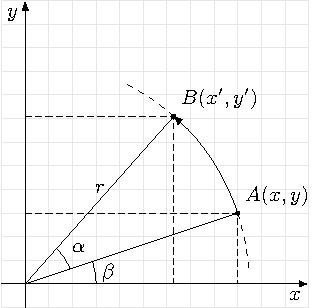
\includegraphics[width=\textwidth]{rotate.pdf}
    	}
    	{
    		
    		$A \rightarrow B$ \\ ~ \\
    		
    		\pause
    		
    		$x'=r\cos (\alpha+\beta)$ \onslide<3->{ $=r(\cos\alpha \cos\beta-\sin\alpha \sin\beta)$}  \\
    		$y'=r\sin (\alpha+\beta)$ \onslide<3->{ $=r(\sin\alpha \cos\beta+\cos\alpha \sin\beta)$} \\~\\
    		
    		\pause[4] 
    		
    		Т.к. $\displaystyle \cos\beta = \frac{x}{r}$ и $\displaystyle\sin\beta=\frac{y}{r}$, то \\ ~ \\
    		
    		$x'=x\cos\alpha-y\sin\alpha$ \\
    		$y'=x\sin\alpha+y\cos\alpha$
    		
    		\pause
    		
    	    \begin{block}{Поворот точки $(x,y)$ на угол $\alpha$}
    	    	$$
    	    	\begin{pmatrix}
    	    		x' \\
    	    		y' \\
    	    	\end{pmatrix}
    	    	=
    	    	\begin{pmatrix}
    	    		\cos\alpha & -\sin\alpha \\
    	    		\sin\alpha & \cos\alpha
    	    	\end{pmatrix}
    	    	\cdot
    	        \begin{pmatrix}
    	    		x \\
    	    		y \\
    	    	\end{pmatrix}
    	    	$$
    	    \end{block}
    		
    		

    	}
    	
    \end{frame}
    
    
    \begin{frame}{Поворот и перемещение}
    	
    	\centering
    	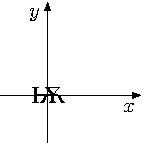
\includegraphics[page=1]{translate4.pdf}
    	\TCT{0.5}
    	{
    		\centering
    		Повернуть --- переместить
    		
    		\includegraphics[page=2]{translate4.pdf}		
    		\includegraphics[page=3]{translate4.pdf}
    	}
    	{
    		\centering
    		Переместить --- повернуть
    		\includegraphics[page=4]{translate4.pdf}		
    		\includegraphics[page=5]{translate4.pdf}
    	}
    	
    \end{frame}
    
    
    \begin{frame}{Поворот точки вокруг другой точки}
    	
    	\TC{0.4}
    	{
    		\only<1>{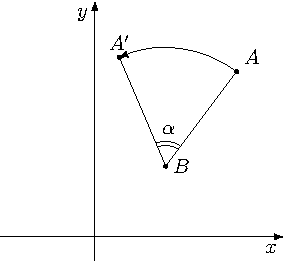
\includegraphics[page=1]{rotate2.pdf}
    		}\only<2>{\includegraphics[page=2]{rotate2.pdf}
    		}\only<3>{\includegraphics[page=3]{rotate2.pdf}
    		}\only<4>{\includegraphics[page=4]{rotate2.pdf}}
    	}
    	{
    		Задача: повернуть точку $A$ вокруг точки $B$ на угол $\alpha$ \\ ~ \\
    		
    		\pause
    		
    		1. Переместить точки $A$ и $B$ на вектор $(-\vv{B})$
    		
    		\pause
    		
    		2. Осуществить поворот точки $A$ на угол $\alpha$
    		
    		\pause
    		
    		3. Выполнить обратный первому шагу перенос.
    	}
    	
    \end{frame}
    
    \subsection{Общий вид матрицы преобразования}
    
    \begin{frame}{Общий вид матрицы преобразования}
    	
    	{
    		\centering
    		
    		$   \textbf{M}=
    			\begin{pmatrix}
    				a&b\\
    				c&d
    			\end{pmatrix}
    		$ \\ ~ \\
    	}
    	
    	\TCT{0.5}
    	{
    		 $
    		\begin{pmatrix}
    			a&c\\
    			b&d
    		\end{pmatrix}
    		\begin{pmatrix}
    			x\\
    			y
    		\end{pmatrix}
    		=
    		\begin{pmatrix}
    			ax+cy \\
    			dy+bx
    		\end{pmatrix}
    		$
    	}
    	{
    		$a$ --- масштабирование по $x$ \\
    		$c$ --- сдвиг по $x$ в единицах $y$\\
    		$d$ --- масштабирование по $y$\\
    		$b$ --- сдвиг по $y$ в единицах $x$
    	} 
    	\hfil \\[2em]
    	
    	Чего не хватает? Безотносительного сдвига по осям:     		
    	$
    	\begin{pmatrix}
    		ax+by+p \\
    		dy+cx+q
    	\end{pmatrix}
    	$    	
    	
    	
    \end{frame}
    
    \begin{frame}{Преобразование единичного квадрата}
    	\TC{0.5}
    	{
    		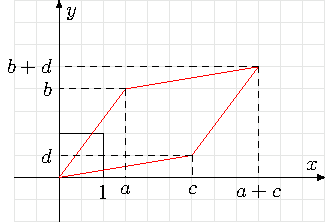
\includegraphics{squere.pdf}
    	}
    	{
    		$\mathbf M =  
    		\begin{pmatrix}
    			a&c\\
    			b&d
    		\end{pmatrix}$
    		
    		$\textbf V = 
    		\begin{pmatrix}
    			0 & 1 & 0 & 1\\
    			0& 0 & 1 & 1
    		\end{pmatrix}$
    		
    		$
    		\textbf V'=\mathbf{MV}=
    		\begin{pmatrix}
    			0 & a & c & (a+c) \\
    			0 & b & d & (b+a)
    		\end{pmatrix}
    		$ \\~\\
    		$S_{V'} = \det(\mathbf M) = ad-bc$
    	}
    \end{frame}
    
    \section{Однородные координаты и матричные операции}
    
    \frame{\sectionpage}
    
    \subsection{Понятие однородных координат}
    
    
    \begin{frame}{Однородные координаты}
    	
    	$(wx,wy,w)$ --- однородные координаты для записи точки на плоскости.
    	$(wx,wy,wz,w)$ --- однородные координаты для записи точки в пространстве.
    	$w$ --- масштабный множитель. \\ ~ \\
    	
    	\pause
    	
    	Для перевода точки в обычные координаты, однородные необходимо разделить на $w$: \\
    	$(wx / w ,wy / w,w /w) \rightarrow (x,y,1)$  \\ ~ \\
    	
    	\pause
    	
    	Некоторые точки, неопределенные в трехмерном пространстве, можно определить в однородных:
    	$(0,0,-\infty) \rightarrow (0,0,1,0)$
    	
    	
    	
    	
    \end{frame}
    
    
	\subsection{Проецирование в однородных координатах}
	
	\FRAME{Проецирование с помощью однородных координат}
	{
		\TC{0.5}
		{
			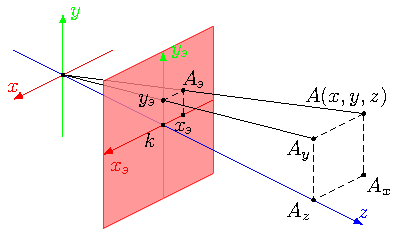
\includegraphics[width=\textwidth]{centralproj2.pdf}
		}
		{
			\def\ekr{\text{\textit{э}}}

			$\displaystyle y_\ekr=\frac{ky}{z}, \ x_\ekr=\frac{kx}{z}$
			
			\pause
			
			Представим, точку в пространстве $(x,y,z)$ в виде однородных координат $(x/z,y/z,1)$ \\ ~ \\
			
			\pause
			
			Тогда, координаты спроецированной на плоскость точки $(x_\ekr, y_\ekr)$ будут совпадать с ее однородными координатами при $k = 1$:
			
			$\displaystyle y = y_\ekr = \frac{y}{z}$ и $\displaystyle x = x_\ekr = \frac{x}{z}$		
			
		}
		
	}
	
	\begin{frame}{Матрица проецирования}
		
		\def\ekr{\text{\textit{э}}}
		$   \textbf{P}=
			\begin{pmatrix}
				k&0&0&0 \\
				0&k&0&0 \\
				0&0&0&0\\
				0&0&1&k
			\end{pmatrix} 
		$ --- матрица центральной проекции.  \\ ~ \\
		
		\pause
		
		Представим точку $v(x,y,z)$ в однородных координатах с помощью матрицы-столбца: 
		$ \textbf{v}=
		\begin{pmatrix}
			wx \\
			wy \\
			wz \\
			w
		\end{pmatrix}
		 $
		 
		\pause
		
		$\textbf{P}\textbf{v}=
		\begin{pmatrix}
			k&0&0&0 \\
			0&k&0&0 \\
			0&0&0&0\\
			0&0&1&k
		\end{pmatrix} 
		\begin{pmatrix}
			wx \\
			wy \\
			wz \\
			w
		\end{pmatrix}
		= 
		\begin{pmatrix}
			kwx \\
			kwy \\
			0 \\
			w(z+k)
		\end{pmatrix} $ \pause
		$
		=
		\begin{pmatrix}
			kx/(z+k) \\
			ky/(z+k) \\
			0 \\
			1
		\end{pmatrix}
		$
		\fbox{
		$
		\begin{matrix}
			\text{\footnotesize С слайда \ref{slide:projection}} \\
			y_\ekr=\frac{ky}{z+k} \\
			x_\ekr=\frac{kx}{z+k}
		\end{matrix}
		$}
	\end{frame}
	
	
	\subsection{Матричные представления двумерных преобразований}
	
	\begin{frame}{Матрица перемещения}
		$
		\begin{pmatrix}
			1&0&a\\
			0&1&b\\
			0&0&1
		\end{pmatrix}
		\begin{pmatrix}
			x\\
			y\\
			1
		\end{pmatrix}
		$ \pause
		$
		=
		\begin{pmatrix}
			x+a\\
			y+b\\
			1
		\end{pmatrix}
		$		
		
		\pause
		
		\begin{block}{Перемещение точки $(x,y)$ на вектор $(a,b)$}
			$$
					\begin{pmatrix}
						x'\\
						y'\\
						1
					\end{pmatrix}
					=
					\begin{pmatrix}
						1&0&a\\
						0&1&b\\
						0&0&1
					\end{pmatrix}
					\cdot
					\begin{pmatrix}
						x\\
						y\\
						1
					\end{pmatrix}
			 $$
		\end{block} 
		
		\begin{block}{Перемещение точки $A$ на вектор $(a,b)$}
			$$
				\textbf{A'} = \textbf{A}\textbf{T}(a,b),
				\text{ где } \textbf{T}(a,b)=					
				{ \footnotesize 
					\begin{pmatrix}
					1&0&a\\
					0&1&b\\
					0&0&1
				\end{pmatrix} 
			   } 
			   \text{--- матрица перемещения}
			$$
		\end{block} 

		
	
		
	\end{frame}



	
	\begin{frame} {Последовательность переносов}
		
		\TC{0.4}
		{
			\only<1-3>{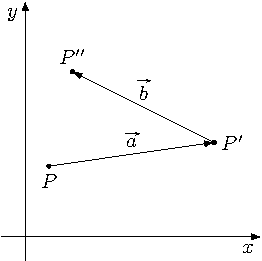
\includegraphics[page=1]{translate2.pdf}
			}\only<4->{\includegraphics[page=2]{translate2.pdf}
			}
			

		}
		{
			$P \xrightarrow{\vv{a}} P' \xrightarrow{\vv{b}} P''$ \\~\\
			
			\pause
			
			$\textbf{P}'=\textbf{T}(\vv{a})\textbf{P}$,\ \ \ $\textbf{P}''=\textbf{T}(\vv{b})\textbf{P}' \Rightarrow $ \\[1em]
			$\Rightarrow \textbf{P}'' = \textbf{T}(\vv{b})\textbf{T}(\vv{a}) \textbf{P}$ \\ ~ \\ 
			
			\pause
			
			$
			   \textbf{T}(\vv{b})\textbf{T}(\vv{a}) = 
			   	\begin{pmatrix}
			   	1&0&b_x\\
			   	0&1&b_y\\
			   	0&0&1
			   \end{pmatrix}  
		       \begin{pmatrix}
			   	1&0&a_x\\
			   	0&1&a_y\\
			   	0&0&1
			   \end{pmatrix} =  
			$ \\ \pause
			$
			=\begin{pmatrix}
				1&0&a_x+b_x\\
				0&1&a_y+b_x\\
				0&0&1
			\end{pmatrix}
			=\textbf{T}(a_x+b_x,a_x+b_y)  
			$
			
			$[P \xrightarrow{\vv{a}} P' \xrightarrow{\vv{b}} P''] \equiv [P \xrightarrow{\vv{a}+\vv{b}} P'']$
			
		}
		

		
  \end{frame}



\begin{frame}{Матрица масштабирования}
	\begin{block}{Матрица масштабирования точки $A$ по вектору $\vv{s}$ }
		$$
			\textbf{A}' =\textbf{S}(s_x,s_y) \textbf{A}, \text{где } \textbf{S}(s_x,s_y) =
			\begin{pmatrix}
				s_x&0&1\\
				0&s_y&1\\
				0&0&1
			\end{pmatrix} 
		$$
	\end{block}
	$
		\begin{pmatrix}
			s_x&0&1\\
			0&s_y&1\\
			0&0&1
		\end{pmatrix}
		\begin{pmatrix}
			x\\
			y\\
			1
		\end{pmatrix}
		=
		\begin{pmatrix}
			xs_x\\
			ys_y\\
			1
		\end{pmatrix}
	$
\end{frame}



\begin{frame}{Последовательность масштабов}

	$	P \xrightarrow{\vv{s}} P' \xrightarrow{\vv{q}} P'' $ \\ ~ \\ \pause
	$	
	    \textbf{S}(\vv{q})\textbf{S}(\vv{s})\textbf{P}=
		\begin{pmatrix}
			q_x&0&1\\
			0&q_y&1\\
			0&0&1
		\end{pmatrix}
		\begin{pmatrix}
			s_x&0&1\\
			0&s_y&1\\
			0&0&1
		\end{pmatrix}
	    \begin{pmatrix}
			x\\
			y\\
			1
		\end{pmatrix}
		=
	$ \\[1em]  \pause
	\hspace{2cm} $   =
		\begin{pmatrix}
			q_xs_x&0&1\\
			0&q_ys_y&1\\
			0&0&1
		\end{pmatrix}
	    \begin{pmatrix}
			x\\
			y\\
			1
		\end{pmatrix}
		= \textbf{S}(\vv{q}*\vv{s})\textbf{P}
	$ \footnote{Поэлементное произведение $\vv{a}*\vv{b}=\vv{c}(a_xa_y,b_xb_y)$}\\[1em]
	
	
	
	$  [	P \xrightarrow{\vv{s}} P' \xrightarrow{\vv{q}} P'' ] \equiv [  P \xrightarrow{\vv{s}*\vv{q}} P''    ]   $
	

\end{frame}



\begin{frame}{Матрица поворота}
	
	\begin{block}{Матрица поворота точки $A$ на угол $\alpha$}
		$$
		\textbf{A}' =\textbf{R}(\alpha) \textbf{A}, \text{где } \textbf{R}(\alpha) =
		\begin{pmatrix}
			\cos\alpha&-\sin\alpha&0\\
			\sin\alpha&\cos\alpha&0\\
			0&0&1
		\end{pmatrix} 
		$$
	\end{block}
	
	$
		\begin{pmatrix}
			\cos\alpha&-\sin\alpha&0\\
			\sin\alpha&\cos\alpha&0\\
			0&0&1
		\end{pmatrix} 
		\begin{pmatrix}
			x\\
			y\\
			1
		\end{pmatrix}
		=
		\begin{pmatrix}
			x\cos\alpha - y\sin\alpha\\
			x\sin\alpha + y\cos\alpha\\
			1
		\end{pmatrix}
	$
	
\end{frame}

\begin{frame}{Последовательность поворотов}
	

	
	$	P \xrightarrow{\alpha} P'  \xrightarrow{\beta} P'' $ \\ ~ \\ \pause
	
	$ \textbf{R}(\beta)\textbf{R}(\alpha) \textbf{A} =
	\begin{pmatrix}
		\cos\alpha&-\sin\alpha&0\\
		\sin\alpha&\cos\alpha&0\\
		0&0&1
	\end{pmatrix} 
	\begin{pmatrix}
		\cos\beta&-\sin\beta&0\\
		\sin\beta&\cos\beta&0\\
		0&0&1
	\end{pmatrix} 
	\begin{pmatrix}
		x\\
		y\\
		1
	\end{pmatrix}
	=
	$ \pause
	$=
	\begin{pmatrix}
		\cos\alpha\cos\beta - \sin\alpha\sin\beta & -\cos\alpha\sin\beta - \sin\alpha\cos\beta & 0 \\
		\sin\alpha\cos\beta + \cos\alpha\sin\beta & -\sin\alpha\sin\beta + \cos\alpha\cos\beta & 0 \\
		0 & 0 & 1
	\end{pmatrix}
	\begin{pmatrix}
		x\\
		y\\
		1
	\end{pmatrix}
	=
	$ \pause
	$
	=
	\begin{pmatrix}
		\cos(\alpha+\beta)&-\sin(\alpha+\beta)&0\\
		\sin(\alpha+\beta)&\cos(\alpha+\beta)&0\\
		0&0&1
	\end{pmatrix} 
	\begin{pmatrix}
	x\\
	y\\
	1
	\end{pmatrix}
	= \textbf{R}(\alpha + \beta)\textbf{A}
	$ \\[1em]
	$ [	P \xrightarrow{\alpha} P' \xrightarrow{\beta} P'' ] \equiv [P \xrightarrow{\alpha+\beta} P'']$ 
	
	
\end{frame}


\begin{frame}{Обратные операции}
	
     \centering
     
     $A \xrightarrow{\text Ѣ} A' \xrightarrow{-\text Ѣ} A'' \ \  \Rightarrow \ \ A = A'' $	\\ ~ \\ \pause
     
    \centering
     <<Честные>> обратные операции\\ ~ \\
     
     \begin{columns}[T]
     	\begin{column}{0.29\textwidth}
     	   
     	   \footnotesize  
     	   1. Перемещение
     		
     		$\textbf{T}(\vv a)=
     		\begin{pmatrix}
     			1&0&a_x\\
     			0&1&a_y\\
     			0&0&1
     		\end{pmatrix}$ \\
     		
     		$\textbf{T}(-\vv a)=
     		\begin{pmatrix}
     			1&0&-a_x\\
     			0&1&-a_y\\
     			0&0&1
     		\end{pmatrix}$   
     	\end{column}
     	\begin{column}{0.4\textwidth}
     		\scriptsize 
     		
     		2. Поворот
     		 
     		 $\textbf{R}(\alpha)=
     		\begin{pmatrix}
     			\cos\alpha&-\sin\alpha&0\\
     			\sin\alpha&\cos\alpha&0\\
     			0&0&1
     		\end{pmatrix}$ \\
     		
     		 $\textbf{R}(-\alpha)=
			\begin{pmatrix}
				\cos(-\alpha)\!&\! -\sin(-\alpha)\!&\! 0\\
				\sin(-\alpha)\!&\! \cos(-\alpha)\!&\! 0\\
				0\!&\! 0\!&\! 1
			\end{pmatrix}$ 
     	\end{column}
     	\begin{column}{0.32\textwidth}
     		\footnotesize
     		3. Масштабирование
     		$
     		\textbf{S}(s_x,s_y)=
     		\begin{pmatrix}
     			s_x&0&0\\
     			0&s_y&0\\
     			0&0&1
     		\end{pmatrix}
     		$
     		
     		$
     		\textbf{S}(\frac{1}{s_x},\frac{1}{s_y})=
     		\begin{pmatrix}
     			\frac{1}{s_x}&0&0\\
     			0&\frac{1}{s_y}&0\\
     			0&0&1
     		\end{pmatrix}
     		$
     	\end{column} 
     	
     
     \end{columns}
     
     
     ~ \\ \pause
     
       \centering
       Обратные операции через обратные матрицы \\ ~ \\
       
       Если $A = A''$, значит при $\textbf{X}\textbf{A}=\textbf{A}, \ \textbf{X}=\textbf{E}, \  \textbf{E}=\textbf{M}\textbf{M}^{-1}$  \\ 
        $
       \textbf{M}^{-1}\textbf{M}\textbf{A}=\textbf{A}
       $
        \pause
       
       \begin{columns}[T]
     	\begin{column}{0.29\textwidth}
     		
		$\textbf{T}(-\vv a )=\textbf{T}^{-1}(\vv a)$
			 
     	\end{column}
     	\begin{column}{0.4\textwidth}
		
		$\textbf{R}(-\alpha )=\textbf{R}^{-1}(\alpha)$
		
     	\end{column}
     	\begin{column}{0.32\textwidth}
      
      	$
      		\textbf{S}(\frac{1}{s_x},\frac{1}{s_y})=\textbf{S}^{-1}(s_x,s_y) 
      	$ 
      	

     	\end{column}
     \end{columns}

\end{frame}

	



\begin{frame}{Комбинация движений}
	\TC{0.4}
	{
		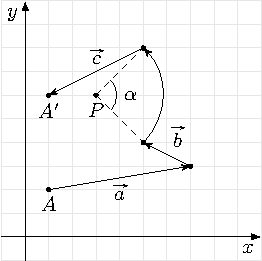
\includegraphics{translate3.pdf}
	}
	{
		$A \rightarrow A' $ \\ ~ \\ \pause
		
		\hspace{1cm}\tikz{\draw [-Latex] (0,0) -- (4.5,0) node [midway,above] {\small Порядок записи}; } \\[0.5em]
		$  \textbf{A}'=\textbf{T}(\vv c)\textbf{T}(\vv P)\textbf{R}(\alpha)\textbf{T}(-\vv P)\textbf{T}(\vv b)\textbf{T}(\vv a)\textbf{A}  $  \\[0.5em] 
		\hspace{1cm}\tikz{\draw [Latex-] (0,0) -- (4.5,0) node [midway,below] {\small Порядок выполнения}; } 
		\\ ~ \\ \pause
		
		$ \textbf{M} = \textbf{T}(\vv c)\textbf{T}(\vv P)\textbf{R}(\alpha)\textbf{T}(-\vv P)\textbf{T}(\vv b)\textbf{T}(\vv a) $ 
		
		$\textbf{A}' = \textbf{M}\textbf{A}$ \\ ~ \\ \pause
		
		$A' \rightarrow A: \ \textbf{A}=\textbf{M}^{-1}\textbf A'$
		
		
	}


\end{frame}



\subsection{Общий вид матрицы преобразования}

\begin{frame}{Общий вид матрицы преобразования}
	
	{
		\centering
		
		$   \textbf{M}=
		\begin{pmatrix}
			a&b&p\\
			c&d&q\\
			l&m&n
		\end{pmatrix}
		$ \\ ~ \\
	}
	

		$
		\begin{pmatrix}
			a&b&p\\
			c&d&q\\
			l&m&n
		\end{pmatrix}
		\begin{pmatrix}
			x\\
			y\\
			1
		\end{pmatrix}
		=
		\begin{pmatrix}
			ax+by+p \\
			dy+cx+q \\
			lx+my+n
		\end{pmatrix}
		=
		\begin{pmatrix}
			(ax+by+p)/(lx+my+n) \\
			(dy+cx+q)/(lx+my+n) \\
			1
		\end{pmatrix}		
		$ \\ ~ \\

		$a$ --- масштабирование по $x$ \\
		$b$ --- сдвиг по $x$ в единицах $y$\\
		$d$ --- масштабирование по $y$\\
		$c$ --- сдвиг по $y$ в единицах $x$ \\
		$p$ --- абсолютный сдвиг по $x$ \\
		$q$ --- абсолютный сдвиг по $y$ \\
		$l,m$ --- коэф. проецирования \\
		$n$ --- коэф. глобального масштабирования
	

	
	
\end{frame}


\end{document}